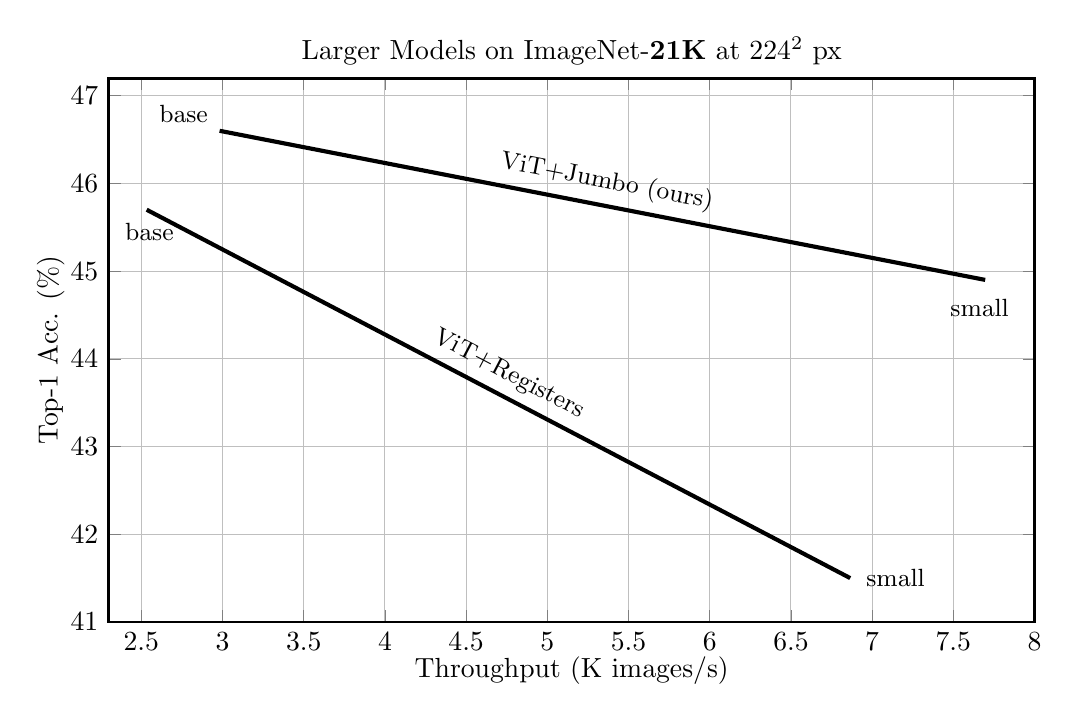
\begin{tikzpicture}
\begin{axis}[
    width=1.1\linewidth,
    height=0.7\linewidth,
    title={Larger Models on ImageNet-\textbf{21K} at $224^2$ px},
    title style={yshift=-5pt},
    xlabel={Throughput (K images/s)},
    xlabel shift=-5pt,
    ylabel={Top-1 Acc. ($\%$)},
    ylabel shift=-5pt,
    xmin=2.3, xmax=8.0,
    ymin=41., ymax=47.2,
    grid=major,
    line width=1pt
]
    % \shade[
    %     right color=yellow!60,
    %     left color=white,
    %     middle color=white,
    %     samples=100,
    %     opacity=0.2
    % ] (rel axis cs:0,1) -- (rel axis cs:1,1) -- (rel axis cs:1,0) -- cycle;
    
    % \shade[
    %     top color=yellow!60,
    %     bottom color=white,
    %     middle color=white,
    %     samples=100,
    %     opacity=0.2
    % ] (rel axis cs:0,1) -- (rel axis cs:1,1) -- (rel axis cs:1,0) -- cycle;
    
    % \node[anchor=south west] at (rel axis cs:0.82,0.85) {\small optimal};

    % --- Registers line ---
    \draw[\registerColor, line width=1.5pt]
      (axis cs:6.865,41.5) coordinate (B1)
      -- (axis cs:2.533,45.7) coordinate (B2)
      node[midway, above, sloped] {\small ViT+Registers};

    % Place Registers markers at coordinates (with full scale, here 1.0)
    \RegisterMarker[1.2]{(B1)}
    \node[right, \registerColor, xshift=2pt, yshift=0pt] at (B1) {\small small};

    \RegisterMarker[1.2]{(B2)}
    \node[below, \registerColor, xshift=1pt, yshift=-1pt] at (B2) {\small base};

    % --- Jumbo line ---
    \draw[\jumboColor, line width=1.5pt]
      (axis cs:7.696,44.9) coordinate (R1)
      -- (axis cs:2.982,46.6) coordinate (R2)
      node[midway, above, sloped] {\small ViT+Jumbo (ours)};

    \JumboMarker[0.5]{(R1)}
    \node[below, \jumboColor, xshift=-2pt, yshift=-3pt] at (R1) {\small small};

    \JumboMarker[0.5]{(R2)}
    \node[above, \jumboColor, xshift=-13pt, yshift=-1pt] at (R2) {\small base};

\end{axis}
\end{tikzpicture}